\chapter{Comparaison entre le harnais de test et JUnit}
\label{chap:comparaison}

    \begin{figure}[H]
        \begin{center}
          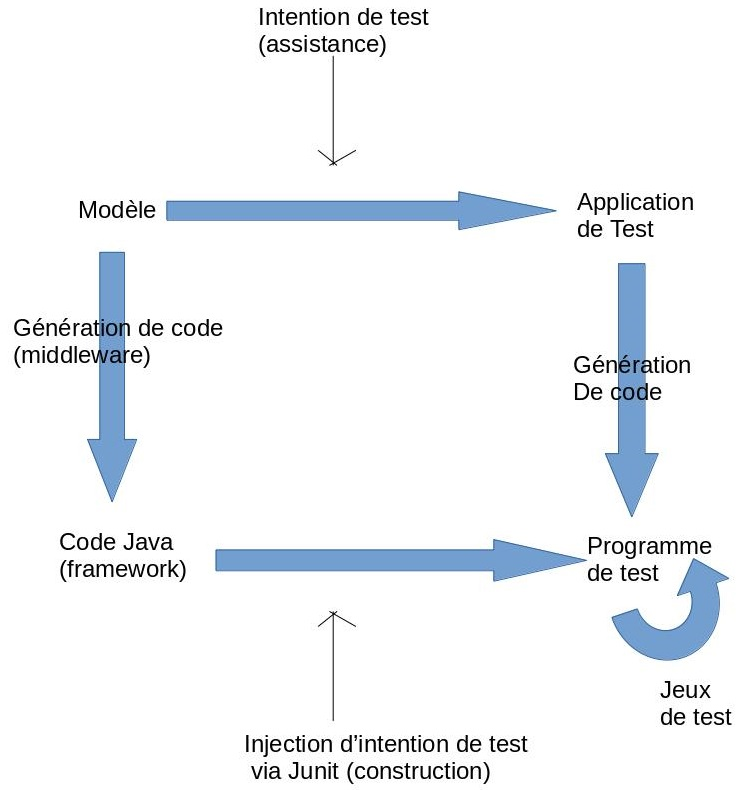
\includegraphics[scale=0.5]{images/structSchema.jpg}
          \label{fig:StructModelTests}
          \caption{Structure des tests sur le modèle par assistance ou construction}
        \end{center}
    \end{figure} 

Sur la figure ci-dessus, on peut voir les deux manières de tester un modèle, soit à la manière du harnais de tests créés par COSTOTest en utilisant les intentions de tests Kmelia, soit comme nous avons cherché à le faire en générant du code conforme au modèle que nous testons ensuite manuellement en injectant nos intentions de tests via JUnit.

L'hypothèse de départ est qu'il est plus rentable en terme de temps de générer les tests sur le modèle et non pas sur le code généré à partir du modèle.

\section{Intérêts du test sur le modèle par rapport à Junit}

Grâce à l'utilisation du générateur de harnais de tests dans COSTOTest en suivant la procédure indiquée dans la documentation, la génération du test de computeSpeed() est relativement rapide à mettre en place, les fonctionnalités du plugin permettant d'intégrer les données multiples en une seule fois grâce à un fichier .csv contenant les données d'entrée et les oracles pour les tests.

De plus, la présence et l'utilisation de frameworks et autres middlewares pour que le programme gère notamment la concurrence et les buffers de communications rend la génération de tests par JUnit plus complexe.

\section{Notre avis}

Après tout le temps passé à comprendre comment fonctionne COSTO, le harnais de test généré, utiliser JUnit nous paraît moins efficace notamment car il faut créer soi-même les mocks que COSTOTest génère automatiquement. 

Cependant malgré la pénibilité de devoir utiliser JUnit ou tout autre framework de test (Mockito, Cobertura, \dots), il reste utile de test le "\textit{produit fini}". 

De manière plus pratique l'avantage de Junit par rapport à Kmelia est que plus personnes sont former à son utilisation et qu'il ne demande pas d'apprendre un nouveau langage.